%input macros (i.e. write your own macros file called MacroFile1.tex)
    %\newcommand{\PdfPsText}[2]{
  \ifpdf
     #1
  \else
     #2
  \fi
}

\newcommand{\IncludeGraphicsH}[3]{
  \PdfPsText{\includegraphics[height=#2]{#1}}{\includegraphics[bb = #3, height=#2]{#1}}
}

\newcommand{\IncludeGraphicsW}[3]{
  \PdfPsText{\includegraphics[width=#2]{#1}}{\includegraphics[bb = #3, width=#2]{#1}}
}

\newcommand{\InsertFig}[3]{
  \begin{figure}[!htbp]
    \begin{center}
      \leavevmode
      #1
      \caption{#2}
      \label{#3}
    \end{center}
  \end{figure}
}


%%% Local Variables: 
%%% mode: latex
%%% TeX-master: "~/Documents/LaTeX/CUEDThesisPSnPDF/thesis"
%%% End: 



\documentclass[oneside,12pt]{CUEDthesisPSnPDF}
\begin{document}

\renewcommand{\thepage}{\mbox{A-\arabic{page}}}
\renewcommand\thechapter{\Alph{chapter}}
\renewcommand{\chaptername}{Appendix}
\renewcommand{\thefigure}{A-\arabic{chapter}.\arabic{figure}}
\renewcommand{\thetable}{A-\arabic{chapter}.\arabic{table}}
\setcounter{page}{22}
\addtocounter{chapter}{2}

\chapter{Process model of monitor}
\thispagestyle{fancy}
\begin{figure}[!htb]
\centering
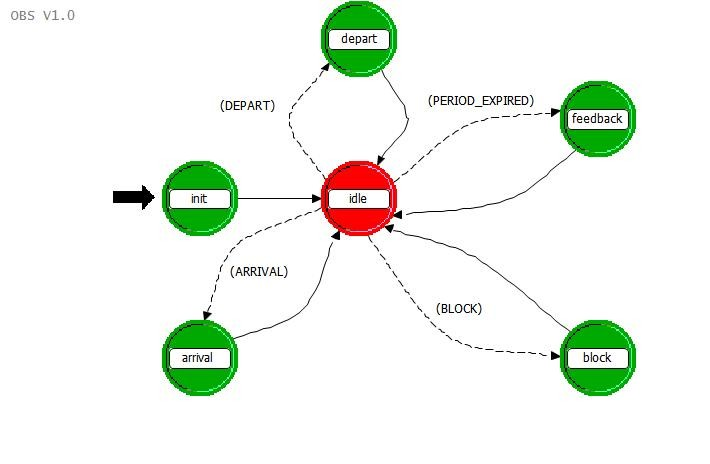
\includegraphics[width=2.6in]{fig/monitor}
\caption{process model of monitor}
\label{fig:monitor}
\end{figure}

The monitor of core node detect each output-port congestion status and broadcast feedback control packet to all associate edge node periodically. As shown in figure \ref{fig:monitor}, it track the number of blocked burst and the number of arrival and departed burst. And there a self interruption as timer.  

\end{document}
